% chap3.tex
\chapter{掌表面の付着水分量の測定と\\
\hspace{4\zw}統計解析}

\section{本章の目的}

本章では、掌が水に接触した際にどの程度の水分が皮膚表面に付着・保持されるのかを
定量的に評価することを目的とした。
手指は日常的に外気やさまざまな物体に触れており、その皮膚状態は温度、湿度、
使用環境などの影響を受けやすい。
そのため、同一人物であっても皮膚の厚さやしわの状態、利き手・非利き手といった
使用頻度の違いによって、水分の付着量に差が生じる可能性が考えられる。

本研究では、右手および左手を同一条件下で水に浸漬し、
一定時間保持した後に引き上げる操作を繰り返すことで、
手の形状や皮膚状態の違いが水分付着量に与える影響を評価した。
さらに、測定動作を可能な限り一定化することで、
時間や手の動かし方による誤差を低減し、
掌表面に保持される水分量をより正確に測定することを試みた。

また、被験者間の個人差を評価するため、
身体的特徴の異なる被験者9名を対象として測定を行い、
後続章におけるウイルス付着量および洗浄後残存量の評価に必要な
基礎データを取得することを本章の目的とした。

%--------------------------------------------------

\section{実験材料}

本研究における掌への水分付着量測定には、
以下の器具および材料を使用した。

\begin{itemize}
  \item 蒸留水（900mL）
  \item トレー（水を保持するため）
  \item 電子天秤（質量変化測定用）
  \item 使い捨て紙タオル
\end{itemize}

測定は外部環境の影響を抑えるため、
風の当たらない室内環境において実施した。

%--------------------------------------------------

\section{掌への水分付着量測定方法}

\subsection{実験条件および測定手順}

測定前に、トレーへ蒸留水900mLを注ぎ、
常に同一水量となるよう調整した。
実験は温度および湿度の影響を受けやすいため、
周囲環境を可能な限り一定に保った状態で実施した。

測定前には、被験者に石けんを用いて手を十分に洗浄させ、
使い捨て紙タオルで水分を拭き取った後、測定を開始した。

測定手順を以下に示す。

\begin{enumerate}
  \item 片方の手を用いて測定を行う。
  \item 手を蒸留水中へ静かに挿入し、手全体が水に浸るようにする。
  \item 約5秒間静止させ、掌全体に水分が均一に付着するようにする。
  \item 手を静かに引き上げ、自然に落下する水滴のみを対象とする。
  \item 手を振るなどの動作は行わず、20秒間静止する。
\end{enumerate}

この操作を右手および左手で交互に行い、
各手について同一条件下で複数回の測定を実施した。

\subsection{秤量による付着水量の算出方法}
手から落下する水滴は、
トレー下部に設置した電子天秤により質量変化として測定した。
20秒間静止後に読み取った質量変化を、
掌に付着した水分量とした。

本測定は、学生8名および教員1名の計9名の被験者を対象として実施し、
各被験者について右手および左手それぞれ25回ずつ測定を行った。
その結果、取得された水分付着量データの総数は
$n = 450$（9名 $\times$ 左右2手 $\times$ 25回）である。

得られた質量値は、水の密度を1.0g/mLと仮定し、
体積（mL）として換算した。

なお、測定結果の一例として、
被験者Aにおける右手および左手の水分付着量の平均値および偏差を
表\ref{tab:water_subjectA}に示す。

\begin{table}[htbp]
  \centering
  \caption{被験者Aにおける掌への水分付着量測定結果（平均値および偏差）}
  \label{tab:water_subjectA}
  \begin{tabular}{lcccc}
    \hline
    被験者 &
    右手平均 (mL) &
    右手偏差 (mL) &
    左手平均 (mL) &
    左手偏差 (mL) \\
    \hline
    A & 1.74 & 0.12 & 1.69 & 0.08 \\
    \hline
  \end{tabular}
\end{table}

%--------------------------------------------------

\section{掌面積による水分付着量の正規化}

本研究では、被験者間の掌の大きさの違いを考慮するため、
第2章で求めた掌面積を用いて水分付着量の正規化を行った。
具体的には、測定された水分付着量を掌面積で除することで、
単位面積あたりの水分付着量を算出した。

この正規化により、掌の大きさに依存しない形で
水分付着特性を比較することが可能となる。

%--------------------------------------------------

\section{統計解析方法}

本研究では、掌に付着する水分量について、左右差および被験者間の個人差を同時に評価するため、
混合効果モデルを用いた解析を行った。混合効果モデルは、繰り返し測定や個人差を含むデータ解析に適した統計手法であり、
評価対象となる要因（固定効果）と、測定対象ごとに生じるばらつき（ランダム効果）を同一のモデル内で扱うことができる。
本解析では、左右の掌の別を固定効果とし、被験者ごとの水分付着量の違いをランダム効果としてモデル化した。
これは、皮膚の状態や水切りの癖など、測定や制御が困難な被験者固有の要因による影響を統計的に考慮するためである。

\subsection{解析モデル}
水分付着量（$mL/cm^2$）を目的変数とし、以下の混合効果モデルを構築した。
\begin{itemize}
    \item 固定効果: 手の別（右手、左手）
    \item ランダム効果: 被験者（9名）
\end{itemize}

\subsection{解析結果}

混合効果モデルによる解析結果を以下に示す。

固定効果において、左手を基準とした場合の右手との差（HandRight）は
$2.59 \times 10^{-5}\,\mathrm{mL/cm^2}$ と推定され、その差は極めて小さかった。
また、この左右差に対する検定の結果、$p = 0.707$ となり、
統計的に有意な差は認められなかった。

一方、ランダム効果として設定した被験者間のばらつきには一定の大きさが認められた。
被験者間の標準偏差は約 $0.0010\,\mathrm{mL/cm^2}$、
同一被験者内の測定誤差の標準偏差は約 $0.00073\,\mathrm{mL/cm^2}$ であり、
水分付着量には被験者間の個人差が存在することが示唆された。

以上の結果より、水分付着量は被験者によって異なる傾向がある一方で、
同一被験者内における左右の掌の違いは統計的に有意ではないことが明らかとなった。
すなわち、水分付着量のばらつきは左右差よりも、
被験者固有の要因によって主に規定されていると考えられる。

このことから、掌面積による補正を行った後においても個人差は残存するものの、
左右差の影響は小さく、実質的に無視できる範囲であると判断される。

本解析により、水分付着量の評価において左右を区別して扱う必要性は低いことが示された。
この結果は、以降のウイルス付着量や残存率、
感染リスク評価に関する解析において、
左右の掌を統合して取り扱うことの妥当性を支持するものである。

また、被験者間の個人差が統計的に確認されたことは、
今後のリスク評価において、
水分付着量を単一の値ではなく、
分布として扱う必要性を示唆している。

\subsection{水分付着量データの分布特性}

混合効果モデルの解析結果より、左右の掌における水分付着量に
統計的に有意な差は認められなかったため、
本節では左右および被験者の測定値を統合した
水分付着量データについて分布特性の検討を行った。

統合した水分付着量データに対して正規確率紙（QQプロット）を作成した結果、
図\ref{fig:qq_water_attachment}に示すように、
データ点は概ね直線上に分布しており、
分布形は正規分布から大きく逸脱していないことが確認された。
\begin{figure}[htbp]
  \centering
  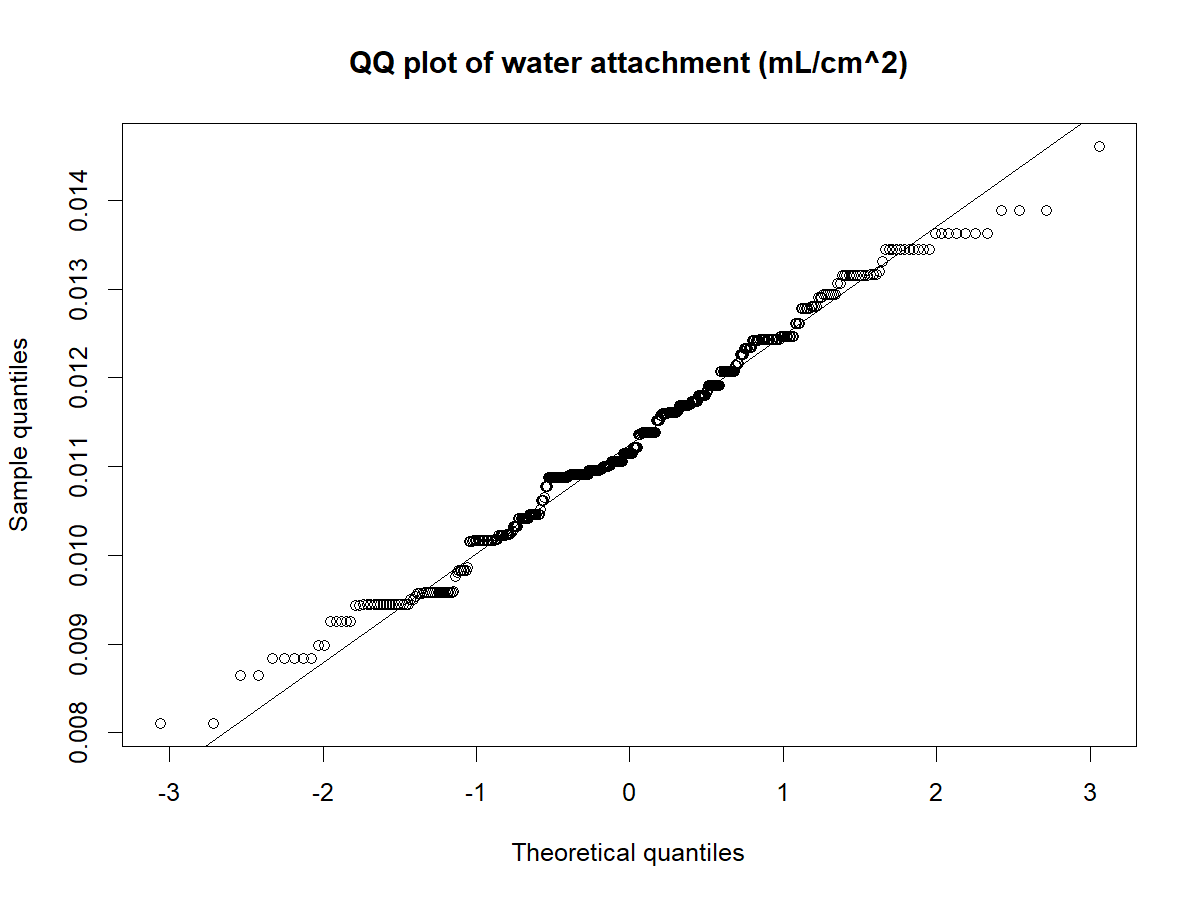
\includegraphics[width=0.7\linewidth]{fig/QQplot_water_attachment.png}
  \caption{水分付着量（mL/cm$^2$）の正規確率紙（QQプロット）}
  \label{fig:qq_water_attachment}
\end{figure}


このことから、
水分付着量（mL/cm$^2$）は、
平均値 $\mu = 0.01128\,\mathrm{mL/cm^2}$、
標準偏差 $\sigma = 0.00119\,\mathrm{mL/cm^2}$ をもつ
正規分布に概ね従うものと判断した。またその分布形を図\ref{fig:hist_water_attachment}に示す。

\begin{figure}[H]
  \centering
  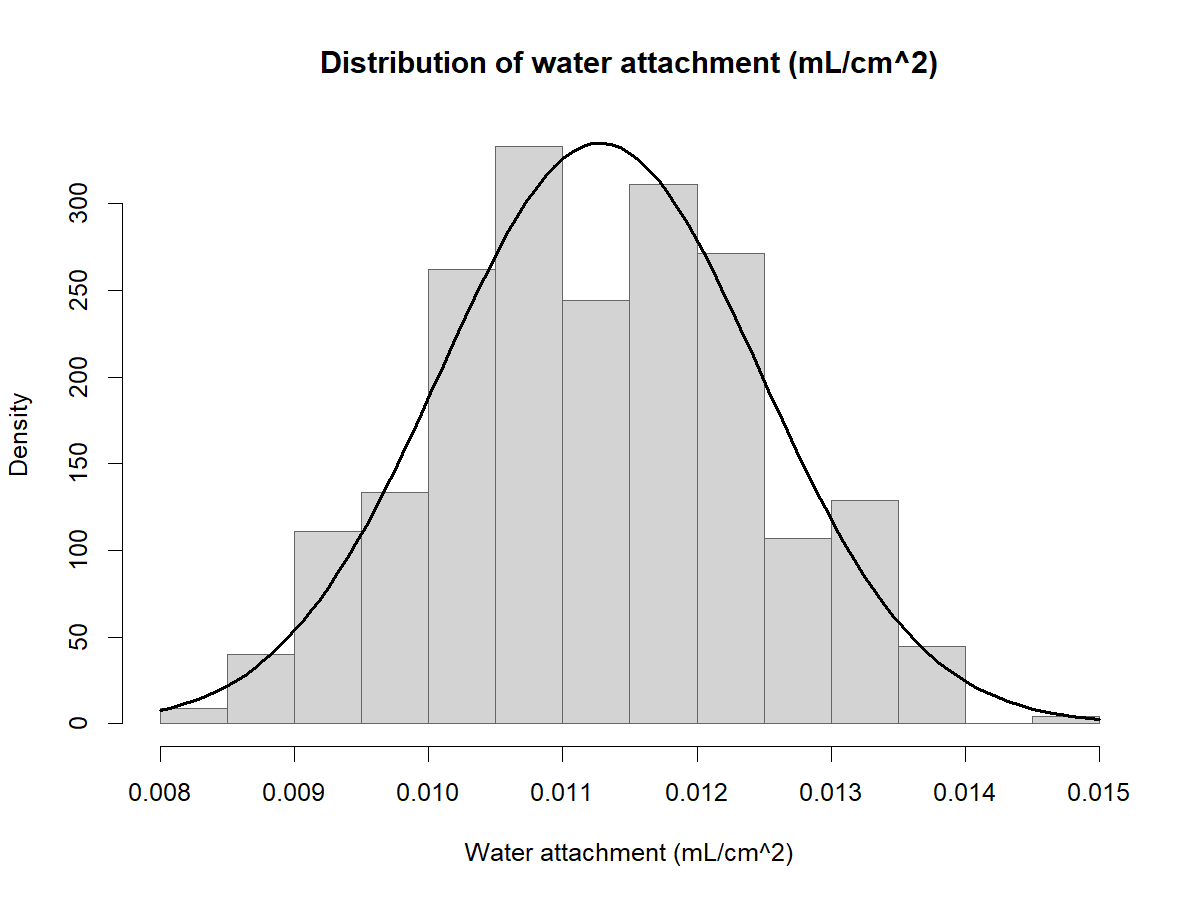
\includegraphics[width=0.7\linewidth]{fig/Histogram_water_attachment_normal.png}
  \caption{%
    水分付着量（mL/cm$^2$）の分布（ヒストグラム）および正規分布曲線\\
    \hspace*{5em}%
    （平均値 $\mu = 0.01128\,\mathrm{mL/cm^2}$，
    標準偏差 $\sigma = 0.00119\,\mathrm{mL/cm^2}$）
  }
  \label{fig:hist_water_attachment}
\end{figure}

%--------------------------------------------------

\section{本章のまとめ}

本章では、掌が水に接触した際の水分付着量を
定量的に測定する手法を確立した。
得られた結果から、水分付着量には
被験者間および左右の手において
一定のばらつきが認められたものの、
全体として大きな個人差は確認されなかった。

